% Options for packages loaded elsewhere
\PassOptionsToPackage{unicode}{hyperref}
\PassOptionsToPackage{hyphens}{url}
\PassOptionsToPackage{dvipsnames,svgnames,x11names}{xcolor}
%
\documentclass[
  12pt]{article}

\usepackage{amsmath,amssymb}
\usepackage{iftex}
\ifPDFTeX
  \usepackage[T1]{fontenc}
  \usepackage[utf8]{inputenc}
  \usepackage{textcomp} % provide euro and other symbols
\else % if luatex or xetex
  \usepackage{unicode-math}
  \defaultfontfeatures{Scale=MatchLowercase}
  \defaultfontfeatures[\rmfamily]{Ligatures=TeX,Scale=1}
\fi
\usepackage{lmodern}
\ifPDFTeX\else  
    % xetex/luatex font selection
\fi
% Use upquote if available, for straight quotes in verbatim environments
\IfFileExists{upquote.sty}{\usepackage{upquote}}{}
\IfFileExists{microtype.sty}{% use microtype if available
  \usepackage[]{microtype}
  \UseMicrotypeSet[protrusion]{basicmath} % disable protrusion for tt fonts
}{}
\makeatletter
\@ifundefined{KOMAClassName}{% if non-KOMA class
  \IfFileExists{parskip.sty}{%
    \usepackage{parskip}
  }{% else
    \setlength{\parindent}{0pt}
    \setlength{\parskip}{6pt plus 2pt minus 1pt}}
}{% if KOMA class
  \KOMAoptions{parskip=half}}
\makeatother
\usepackage{xcolor}
\setlength{\emergencystretch}{3em} % prevent overfull lines
\setcounter{secnumdepth}{5}
% Make \paragraph and \subparagraph free-standing
\makeatletter
\ifx\paragraph\undefined\else
  \let\oldparagraph\paragraph
  \renewcommand{\paragraph}{
    \@ifstar
      \xxxParagraphStar
      \xxxParagraphNoStar
  }
  \newcommand{\xxxParagraphStar}[1]{\oldparagraph*{#1}\mbox{}}
  \newcommand{\xxxParagraphNoStar}[1]{\oldparagraph{#1}\mbox{}}
\fi
\ifx\subparagraph\undefined\else
  \let\oldsubparagraph\subparagraph
  \renewcommand{\subparagraph}{
    \@ifstar
      \xxxSubParagraphStar
      \xxxSubParagraphNoStar
  }
  \newcommand{\xxxSubParagraphStar}[1]{\oldsubparagraph*{#1}\mbox{}}
  \newcommand{\xxxSubParagraphNoStar}[1]{\oldsubparagraph{#1}\mbox{}}
\fi
\makeatother


\providecommand{\tightlist}{%
  \setlength{\itemsep}{0pt}\setlength{\parskip}{0pt}}\usepackage{longtable,booktabs,array}
\usepackage{calc} % for calculating minipage widths
% Correct order of tables after \paragraph or \subparagraph
\usepackage{etoolbox}
\makeatletter
\patchcmd\longtable{\par}{\if@noskipsec\mbox{}\fi\par}{}{}
\makeatother
% Allow footnotes in longtable head/foot
\IfFileExists{footnotehyper.sty}{\usepackage{footnotehyper}}{\usepackage{footnote}}
\makesavenoteenv{longtable}
\usepackage{graphicx}
\makeatletter
\def\maxwidth{\ifdim\Gin@nat@width>\linewidth\linewidth\else\Gin@nat@width\fi}
\def\maxheight{\ifdim\Gin@nat@height>\textheight\textheight\else\Gin@nat@height\fi}
\makeatother
% Scale images if necessary, so that they will not overflow the page
% margins by default, and it is still possible to overwrite the defaults
% using explicit options in \includegraphics[width, height, ...]{}
\setkeys{Gin}{width=\maxwidth,height=\maxheight,keepaspectratio}
% Set default figure placement to htbp
\makeatletter
\def\fps@figure{htbp}
\makeatother

\addtolength{\oddsidemargin}{-.5in}%
\addtolength{\evensidemargin}{-1in}%
\addtolength{\textwidth}{1in}%
\addtolength{\textheight}{1.7in}%
\addtolength{\topmargin}{-1in}%
\makeatletter
\@ifpackageloaded{caption}{}{\usepackage{caption}}
\AtBeginDocument{%
\ifdefined\contentsname
  \renewcommand*\contentsname{Table of contents}
\else
  \newcommand\contentsname{Table of contents}
\fi
\ifdefined\listfigurename
  \renewcommand*\listfigurename{List of Figures}
\else
  \newcommand\listfigurename{List of Figures}
\fi
\ifdefined\listtablename
  \renewcommand*\listtablename{List of Tables}
\else
  \newcommand\listtablename{List of Tables}
\fi
\ifdefined\figurename
  \renewcommand*\figurename{Figure}
\else
  \newcommand\figurename{Figure}
\fi
\ifdefined\tablename
  \renewcommand*\tablename{Table}
\else
  \newcommand\tablename{Table}
\fi
}
\@ifpackageloaded{float}{}{\usepackage{float}}
\floatstyle{ruled}
\@ifundefined{c@chapter}{\newfloat{codelisting}{h}{lop}}{\newfloat{codelisting}{h}{lop}[chapter]}
\floatname{codelisting}{Listing}
\newcommand*\listoflistings{\listof{codelisting}{List of Listings}}
\makeatother
\makeatletter
\makeatother
\makeatletter
\@ifpackageloaded{caption}{}{\usepackage{caption}}
\@ifpackageloaded{subcaption}{}{\usepackage{subcaption}}
\makeatother

\ifLuaTeX
  \usepackage{selnolig}  % disable illegal ligatures
\fi
\usepackage[]{natbib}
\bibliographystyle{agsm}
\usepackage{bookmark}

\IfFileExists{xurl.sty}{\usepackage{xurl}}{} % add URL line breaks if available
\urlstyle{same} % disable monospaced font for URLs
\hypersetup{
  pdftitle={DOGE Days on Reddit: Decoding Public Sentiment in a Federal Shakeup},
  pdfauthor={Kevin Linares; Felix Baez-Santiago; Aria Lu; Gloria Zhou},
  pdfkeywords={Reddit, Federal Government, DOGE},
  colorlinks=true,
  linkcolor={blue},
  filecolor={Maroon},
  citecolor={Blue},
  urlcolor={Blue},
  pdfcreator={LaTeX via pandoc}}



\begin{document}


\def\spacingset#1{\renewcommand{\baselinestretch}%
{#1}\small\normalsize} \spacingset{1}


%%%%%%%%%%%%%%%%%%%%%%%%%%%%%%%%%%%%%%%%%%%%%%%%%%%%%%%%%%%%%%%%%%%%%%%%%%%%%%

\date{April 7, 2025}
\title{\bf DOGE Days on Reddit: Decoding Public Sentiment in a Federal
Shakeup}
\author{
Kevin Linares\\
University of Maryland\\
and\\Felix Baez-Santiago\\
and\\Aria Lu\\
and\\Gloria Zhou\\
University of Michigan\\
}
\maketitle

\bigskip
\bigskip
\begin{abstract}
This study investigates public sentiment on Reddit towards the
Department of Government Efficiency's (DOGE) federal workforce
reduction. Analyzing 400 labeled Reddit comments, we employed supervised
learning (KNN, Random Forest) and unsupervised Large Language Models
(LLMs: Llama 3.2 3B, deepseek-r1:8b) to classify comment stance (favor,
neutral, oppose). While LLMs showed higher precision for opposing
comments, all models struggled with neutral and favoring stances.
Agreement between the two LLMs was fair (Cohen's Kappa = 0.344),
indicating divergent interpretations. Results suggest that accurately
decoding nuanced public sentiment in this context remains challenging
for both traditional and large language models.
\end{abstract}

\noindent%
{\it Keywords:} Reddit, Federal Government, DOGE
\vfill

\newpage
\spacingset{1.9} % DON'T change the spacing!


\section{Introduction}\label{sec-intro}

Established in January 2025, the Department of Government Efficiency
(DOGE) has significantly reduced the federal workforce by over 280,000
employees, fulfilling a key campaign promise of the new administration.
This has caused widespread concern and anxiety among federal workers
about job security and mental well-being. Questions have also been
raised regarding DOGE's adherence to internal policies. To understand
the impact of DOGE's actions on federal worker perceptions of job
security, we collected 400 reddit comments on topics related to DOGE's
tactics in reducing the federal workforce. Additionally, a team of
researchers labeled each comment as whether the author favored, opposed,
or had a neutral stance concerning how DOGE was implementing these
strategies. In the current study we employ two supervise learning model
to predict, given a set of features, comments on stance. We also employ
an unsupervised large language model (LLM) to detect the stance of these
reddit comments and report model findings.

\section{Methods}\label{sec-meth}

\emph{Data}. We collected Reddit comments from subreddits related to the
topic of interest in early March of 2024. This resulted in 12,553
comments which we preprocessed by removing weblinks, replace special
characters (i.e., replaced ``@'' with ``at''), replaced numeric values
with their spelling, and confirmed the absence of duplicate comments. We
then randomly selected 400 comments (without replacement) and assigned
them to four graduate students for coding, categorizing each comment as
favoring, opposing, or neutral towards DOGE's approach to federal
workforce reductions. Table 1 presents the breakdown in percent of our
the comments we labelled and later use to train and evaluate our machine
learning models. A review of the comments revealed more negative
opinionated statements and reactions.

\begin{longtable}[]{@{}lr@{}}
\caption{Distribution of labeled Reddit comment data.}\tabularnewline
\toprule\noalign{}
outcome & Percent \\
\midrule\noalign{}
\endfirsthead
\toprule\noalign{}
outcome & Percent \\
\midrule\noalign{}
\endhead
\bottomrule\noalign{}
\endlastfoot
favor & 28 \\
neutral & 18 \\
oppose & 54 \\
\end{longtable}

We built two supervised machine learning models, K-nearest neighbor and
random forest, to classify Reddit comments concerning stance on the
current reduction in federal workforce into favor, oppose, or neutral.
For model predictors we used the Reddit score, up-votes, and down-votes
each comment received at the time of the collection. Additionally, we
used the keyword that was used to scrape these data along with the
subreddit where the comment was posted. DISCUSS ADDITIONAL FEATURE
ENGINERRING SUCH AS TEXT EDITING THAT WENT INTO THE MODEL. For the KNN
model, we set the number of neighbors hyperparameter to thhree, and for
the random forest, mtry was kept at a constant two as we did not have
many features in these models. We took an 80/20 split for our
training-testing sets that we used to train each model and evaluate.

In addition to our supervised machine learning models, we also applied
to our data two LLMs, llama 3.2. 3B and deepseek-r1:8b. The llama model,
developed by Meta AI released in February 2023, was designed for
applications requiring low-latency inferencing with limited
computational resources, which means that we were able to also deploy
these models on a local machine with a GPU in addition to using the
\href{https://its.umich.edu/advanced-research-computing/}{Great Lakes
HCP}. This model also excels at text classification which is how we used
it to classify the stance for each comment. Deepseek, developed by Liang
Wenfeng in July 2023 and based on the llama architecture, yet boosts
efficiency improvements that appear to provide advances in reasoning,
logic, while excelling at natural language processing. We choose both of
these LLMs as candidates to test against our supervised approaches
because of their ability to apply locally and reputable performance on
zero-shot classification tasks. Both of these models received the same
prompt and tasked which were developed by the research team to reflect
the utility of classifying stance within our topic of interest. Both
LLMs resulted in not being able to classify five comments each while
they only had one in common with the likely reason being that these
comments did not contain enough useful text for a stance to be derive.

Prompt: ``Is this comment in `favor', `neutral', or `oppose' the
reduction in federal workforce? Provide one word answer only!

Task: ``You have assumed the role of a stakeholder that is presented
with a reddit comment from a likely federal worker related to the
current policies on reducing the federal workforce. Please determine the
author's stance on this topic, and only provide the answer.''

To evaluate model performance we used recall to determine how many of
actual positive cases did the model correctly identify. High recall
indicates that the model can correctly identify positive instances but
is also optimistic and may incorrectly label cases as positive. The
second performance metric we selected is precision, of all the items the
model labels as positive how many are true positive, and high precision
indicates that when the model predicts a case to be positive it is
likely to be correct.

\section{Results}\label{results}

Our machine learning models reveal a mix of performance results in
classifying comments into one of three stance categories. Overall, the
random forest model reduces the test misclassification error against
KNN, yet not by much. The stance oppose tended to have the highest
recall of the three with the random forest model having higher scores:
Of all the oppose cases, the random forest model found 74 percent and
the KNN 64 percent. For the neutral stance, the random forest captured 5
percent and KNN 21 percent. While for the favor stance, the random
forest identified 26 percent and KNN 16 percent (see Figure 1 for these
results). Neither model excelled in how many of the stance categories
identified were right as indicated by the precision scores. KNN slightly
outperformed random forest on the oppose stance having correctly
classified 56 percent vs random forest 51 percent or true oppose cases.
For neutral the performance is worse with random forest correctly
identified 50 percent and KNN 21 percent, and same for favor with random
forest correctly identifying 29 percent and KNN 23 percent.

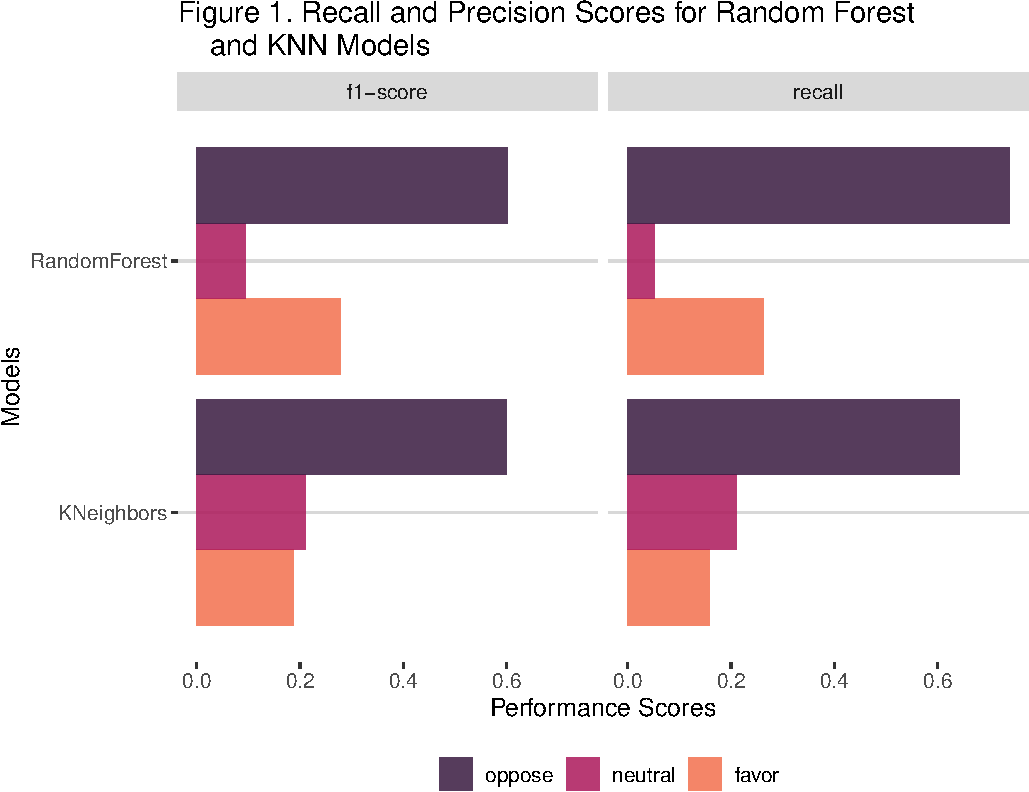
\includegraphics{assign_3_files/figure-pdf/unnamed-chunk-3-1.pdf}

We observe higher precision scores for the oppose stance when using the
LLMs to classify stance positions. Of all the identified oppose stance
cases these models identified, the percent of true oppose cases was 84
percent for llama and 69 percent for deepseek. Similarly, of all the
classified neutral stance classified by these models, the percent of
true neutral cases was 21 percent for llama and 42 percent for deep
seek. Finalkly, of all the identified favor stance, the percent of true
favor cases was 4 percent for llama and 10 percent for deepseek (see
Figure 2 for these results). Recall scores were worse for the oppose
stance, and of all the oppose cases the llama model captured 56 percent
and deepseek 60 percent. For the neutral stance, llama captured 25
percent and deekseek 27 percent. Finally, for the favor stance, llama
captured 29 percent and deekseek 32 percent.

\hfill\break

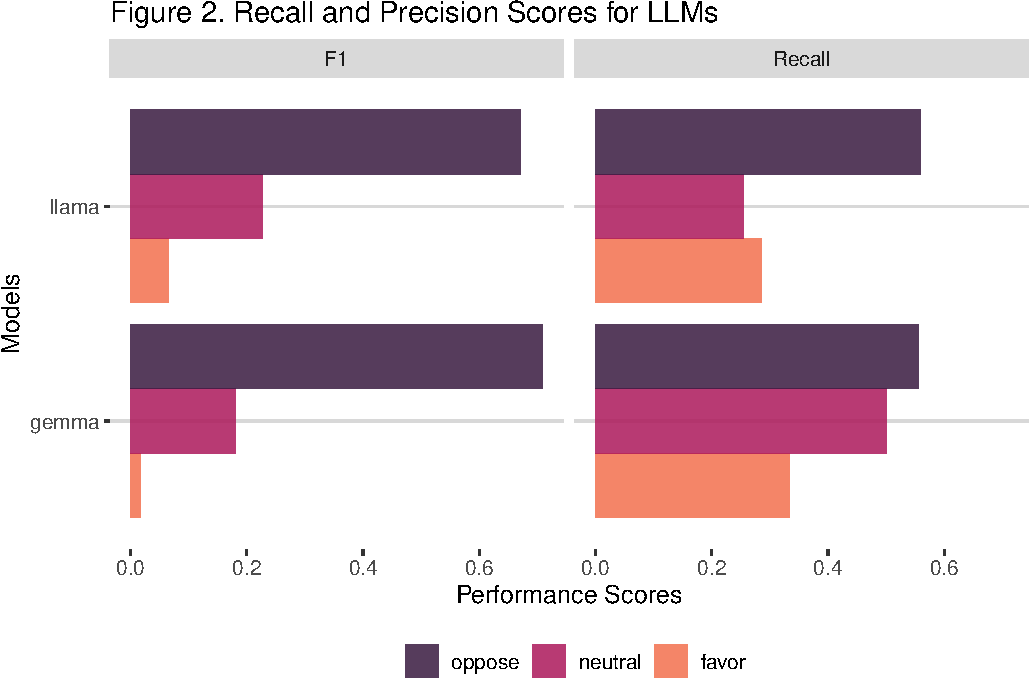
\includegraphics{assign_3_files/figure-pdf/unnamed-chunk-5-1.pdf}

Llama and DeepSeek demonstrated only fair agreement in stance
classification (Cohen's Kappa = 0.344). The contingency table, Table 2
below, reveals highest agreement for ``oppose'' (0.58), indicating some
consistency in identifying strong negative sentiment. However, agreement
was substantially lower for ``neutral'' (0.11) and ``favor'' (0.02),
highlighting divergent interpretations of more nuanced language.
Off-diagonal values further illustrate these discrepancies, suggesting
fundamental differences in how the models process ambiguous cues and
establish classification boundaries, particularly for less extreme
stances.

\begin{longtable}[]{@{}lrrr@{}}
\caption{Aggreement between LLMs, Cohens Kappa, 0.34}\tabularnewline
\toprule\noalign{}
& favor & neutral & oppose \\
\midrule\noalign{}
\endfirsthead
\toprule\noalign{}
& favor & neutral & oppose \\
\midrule\noalign{}
\endhead
\bottomrule\noalign{}
\endlastfoot
favor & 6 & 7 & 1 \\
neutral & 3 & 42 & 14 \\
oppose & 29 & 61 & 228 \\
\end{longtable}

\section{Conclusion}\label{conclusion}

We explored public sentimenton Reddit regarding the DOGE federal
workforce reduction using supervised learning (KNN, Random Forest) and
unsupervised LLMs (Llama 3.2 3B, deepseek-r1:8b) for stance
classification. LLMs showed higher precision for ``oppose'' comments,
suggesting better identification of negative sentiment, but lower
recall, indicating missed opposing comments. Supervised models performed
consistently but generally poorly across all stances, and likely due to
the limited feature set (Reddit metadata) as well as the small sample of
comments.

The consistent difficulty in classifying ``neutral'' and ``favor''
stances across all models likely stems from class imbalance (more
``oppose'' comments), the inherent ambiguity of neutral language, and
potentially more nuanced expressions of favor. The zero-shot approach
for LLMs might also limit their performance on this specific domain. The
few unclassifiable comments highlight the inherent challenges in stance
detection within informal online text.

We conclude that while LLMs showed promise for identifying strong
negative sentiment, accurately classifying the full spectrum of public
opinion on Reddit regarding DOGE's actions remains challenging. Future
research should focus on incorporating richer text-based features for
supervised models, addressing class imbalance, and potentially
fine-tuning LLMs to better capture the nuances of online sentiment and
stance.




\end{document}
